\section{VPN on MacOSX}

Setting up a VPN on MacOSX is very easy once you have your account
details ready, Let's assume have your credentials from your VPN provider
for L2TP/IPSec connection ready. This information should contain the
following:

\begin{itemize}
\item
  Username, ex. \verb!bill2!
\item
  Password, ex. \verb!verysecretpassword!
\item
  VPN server, ex. \verb!tunnel.greenhost.nl!
\item
  A Pre-Shared-Key or Machine-certificate
\end{itemize}
\subsection{Setup}

\begin{enumerate}[1.]
\item
  Before getting started, please be sure you've read the paragraph
  ``testing before and after account set up'', this way you will be able
  to validate if your connection is actually working after set up.
\item
  A VPN is configured in the network settings, that are accessible via
  ``System Preferences..'' in the Apple menu.
\end{enumerate}
\begin{figure}[htbp]
\centering
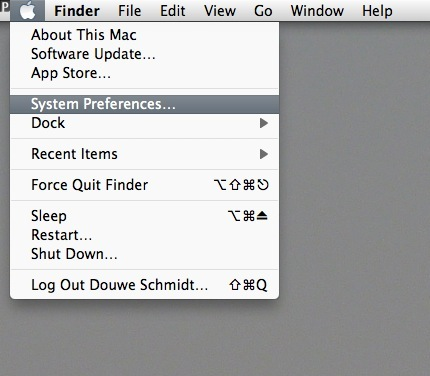
\includegraphics{vpn_osx_02.jpg}
\caption{VPN on Mac OS X}
\end{figure}

\begin{enumerate}[1.]
\setcounter{enumi}{2}
\item
  Next, open the Network preferences.
\end{enumerate}
\begin{figure}[htbp]
\centering
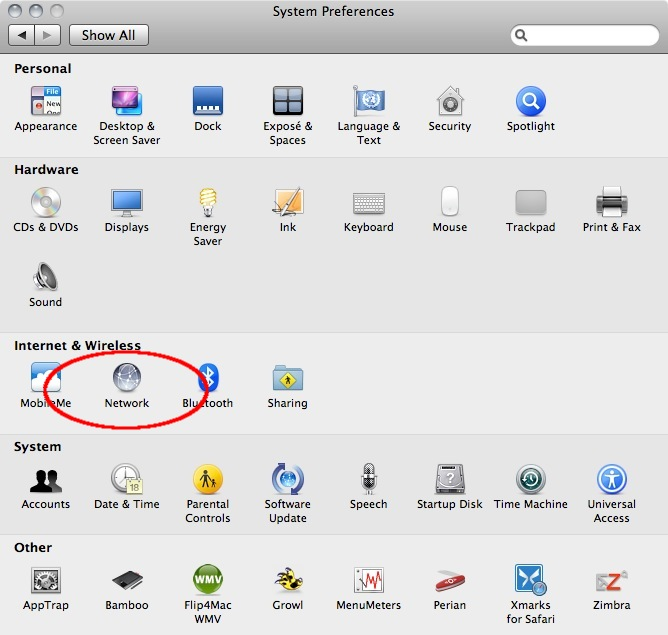
\includegraphics{vpn_osx_03.jpg}
\caption{VPN on Mac OS X}
\end{figure}

\begin{enumerate}[1.]
\setcounter{enumi}{3}
\item
  OSX uses this nifty system to lock windows. To add a VPN it is
  necessary to unlock the screen: you can do this by clicking on the
  lock on the left bottom of the screen.
\end{enumerate}
\begin{figure}[htbp]
\centering
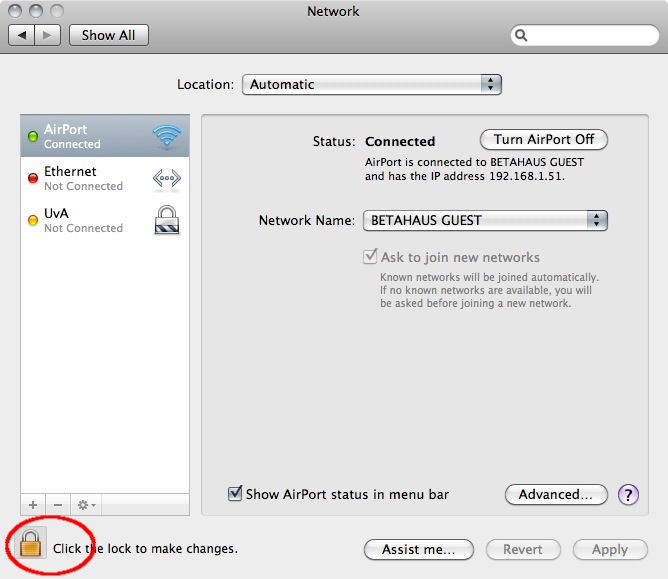
\includegraphics{vpn_osx_04.jpg}
\caption{VPN on Mac OS X}
\end{figure}

\begin{enumerate}[1.]
\setcounter{enumi}{4}
\item
  Enter our user credentials
\end{enumerate}
\begin{figure}[htbp]
\centering
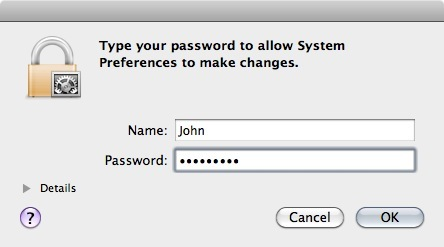
\includegraphics{vpn_osx_05.jpg}
\caption{VPN on Mac OS X}
\end{figure}

\begin{enumerate}[1.]
\setcounter{enumi}{5}
\item
  Now we can add a new network. Do this by clicking on the ``+'' sign
\end{enumerate}
\begin{figure}[htbp]
\centering
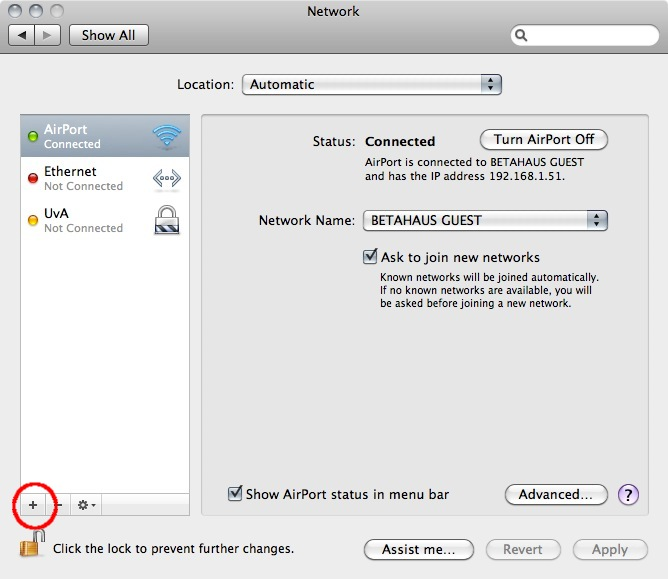
\includegraphics{vpn_osx_06.jpg}
\caption{VPN on Mac OS X}
\end{figure}

\begin{enumerate}[1.]
\setcounter{enumi}{6}
\item
  In the pop-up you need to specify the type of connection. In this case
  choose an VPN interface with L2TP over IPSec. This is the most common
  system. Also don't forget to give the connection a nice name.
\end{enumerate}
\begin{figure}[htbp]
\centering
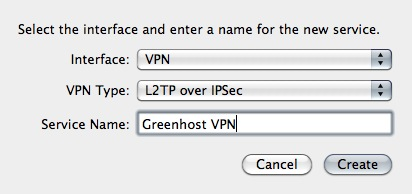
\includegraphics{vpn_osx_07.jpg}
\caption{VPN on Mac OS X}
\end{figure}

\begin{enumerate}[1.]
\setcounter{enumi}{7}
\item
  Next comes the connection data. Please fill in the provided server
  name and user name (called `Account Name'). If this is done, click on
  the ``Authentication Settings\ldots{}'' button
\end{enumerate}
\begin{figure}[htbp]
\centering
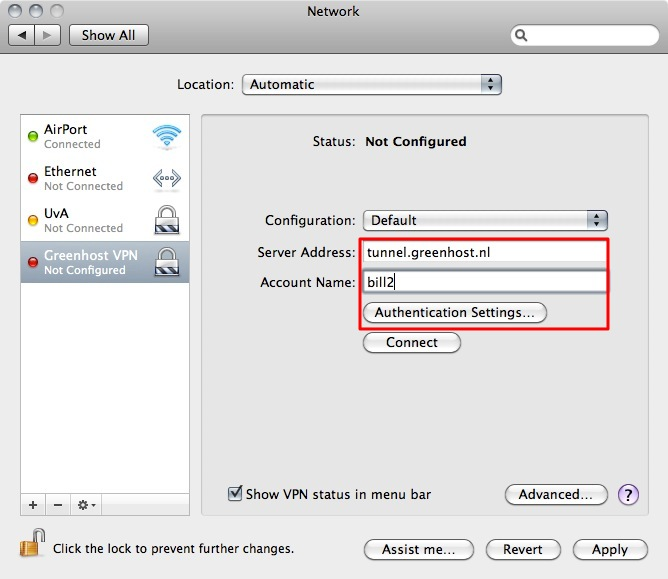
\includegraphics{vpn_osx_08.jpg}
\caption{VPN on Mac OS X}
\end{figure}

\begin{enumerate}[1.]
\setcounter{enumi}{8}
\item
  In the new pop-up you can specify connection specific information.
  This is the way the user is authenticated and how the machine is
  authenticated. The user is very commonly authenticated by using a
  password, although other methods are possible. Machine authentication
  is often done by a Shared Secret (Pre-Shared-Key/PSK), but also quite
  often by using a certificate. In this case we use the Shared Secret
  method. When this is done click OK.
\end{enumerate}
\begin{figure}[htbp]
\centering
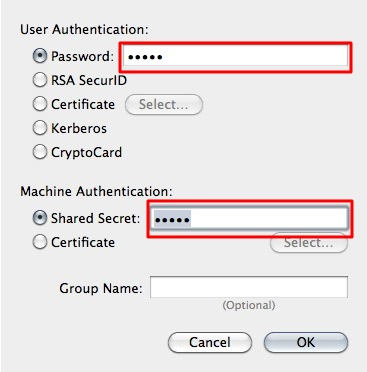
\includegraphics{vpn_osx_09.jpg}
\caption{VPN on Mac OS X}
\end{figure}

\begin{enumerate}[1.]
\setcounter{enumi}{9}
\item
  Now you return back to the network screen. The next step is very
  important, so click on ``Advanced\ldots{}''
\end{enumerate}
\begin{figure}[htbp]
\centering
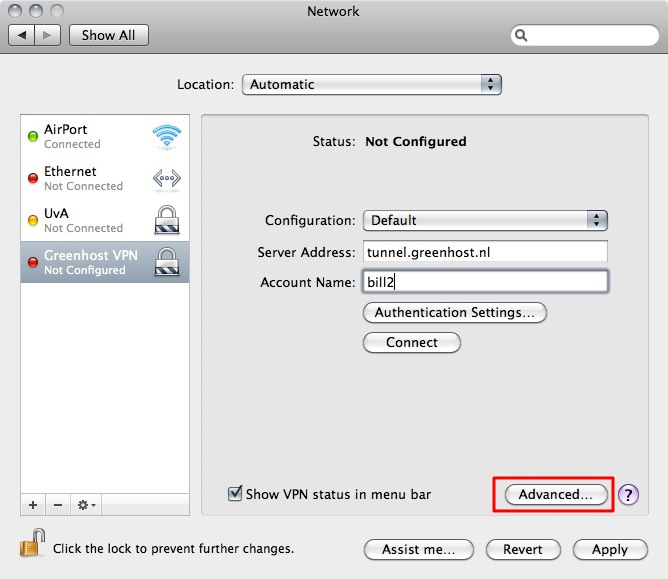
\includegraphics{vpn_osx_09b.jpg}
\caption{VPN on Mac OS X}
\end{figure}

\begin{enumerate}[1.]
\setcounter{enumi}{10}
\item
  In the new pop up you will see an option to route all traffic through
  the VPN connection. We want to enable this, so all our traffic is
  encrypted.
\end{enumerate}
\begin{figure}[htbp]
\centering
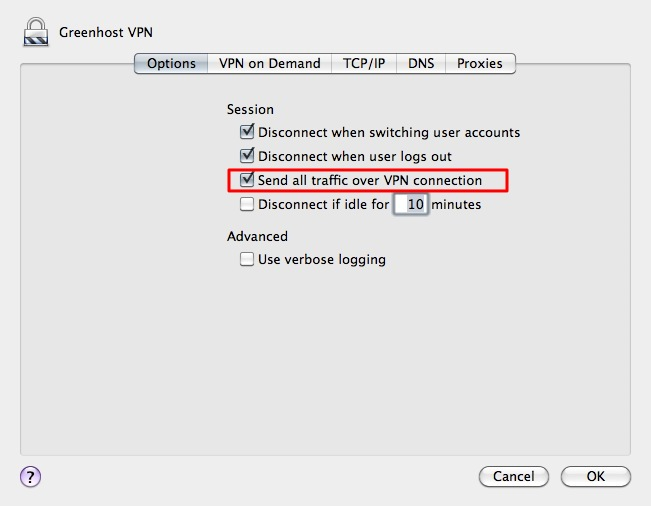
\includegraphics{vpn_osx_10.jpg}
\caption{VPN on Mac OS X}
\end{figure}

\begin{enumerate}[1.]
\setcounter{enumi}{11}
\item
  Well, all is done. Now hit the Connect button!
\end{enumerate}
\begin{figure}[htbp]
\centering
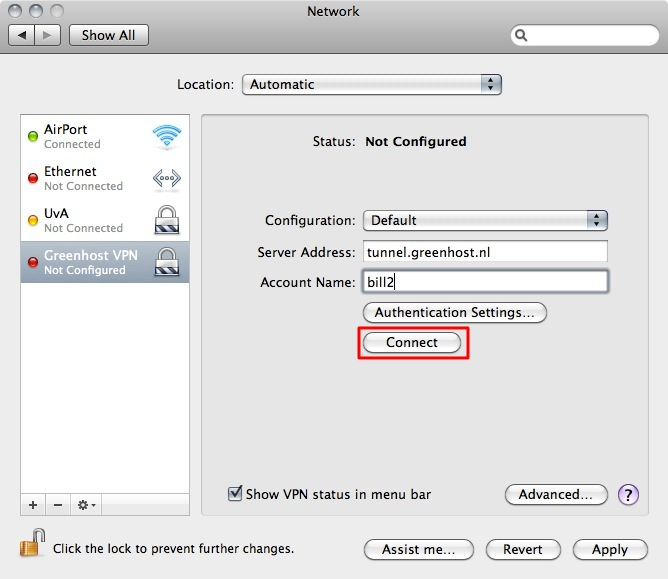
\includegraphics{vpn_osx_11.jpg}
\caption{VPN on Mac OS X}
\end{figure}

\begin{enumerate}[1.]
\setcounter{enumi}{12}
\item
  A pop-up appears. You need to confirm your changes, just hit ``Apply''
\end{enumerate}
\begin{figure}[htbp]
\centering

\includegraphics{vpn_osx_12.jpg}
\caption{VPN on Mac OS X}
\end{figure}

\begin{enumerate}[1.]
\setcounter{enumi}{13}
\item
  After a few seconds, on the left side the connection should turn
  green. If so, you are connected!
\end{enumerate}
\begin{figure}[htbp]
\centering
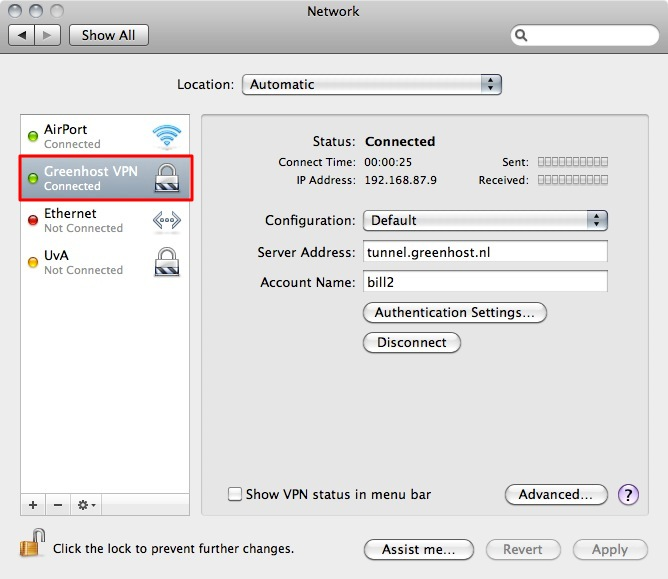
\includegraphics{vpn_osx_13.jpg}
\caption{VPN on Mac OS X}
\end{figure}

\begin{enumerate}[1.]
\setcounter{enumi}{14}
\item
  Ok, now test your connection!
\end{enumerate}
